
%---Define your document class, packages, and new commands

\documentclass[11pt]{article}
\usepackage[top=2.54cm, left=2.54cm, right=2.54cm, bottom=2.54cm]{geometry}

\usepackage{amsfonts}   % for statements to be commented out
\usepackage{amssymb}
\usepackage{amsmath}    % for subequations
\usepackage{setspace}
\usepackage{graphicx}


%------------Document-Begins-Here----------------------%

\begin{document}


\title{\textbf{Orbital Patterns of Martian Moons}}

\author{Jake Mathews
\thanks{mathewsj2@wit.edu}\\
Computer Science Undergraduate Program, Wentworth Institute of Technology\\
550 Huntington Avenue, Boston, MA 02115\\
\and Ian Brown
\thanks{browni1@wit.edu}\\
Computer Engineering Undergraduate Program, Wentworth Institute of Technology\\
550 Huntington Avenue, Boston, MA 02115}

\maketitle

\begin{abstract}

This project's goal was to to create a top-down 2-dimentional model
of the positional path of the moons of Mars, Phobos and Deimos.
We created a Fortran 90 program to simulate the orbit of the two moons
and generate data files for later analysis.
The simulation will be provided some initial conditions of a given moon,
and simulate the orbit over the course of one orbital period, as defined
by NASA~\cite{nasa}

\end{abstract}




% Write your introduction here, include pictures, tables, equations, etc...
\section{Introduction}
An object in orbit is a simple kinematics problem illustrated in Fig.~\ref{fig:centripetal}

\begin{figure}[ht]
  \centering
  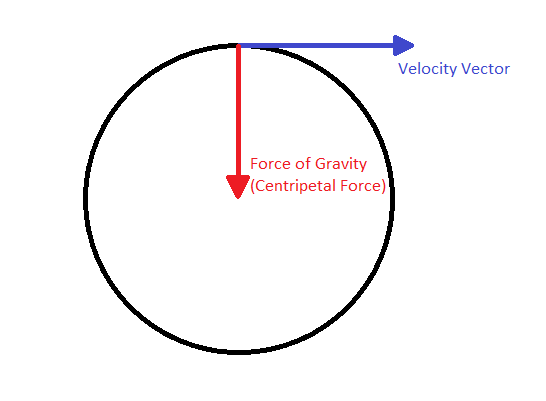
\includegraphics[width=0.6\textwidth, angle =0]{../images/centripetal-force}
  \caption{Centripetal force on an object with a velocity vector}
  \label{fig:centripetal}
\end{figure}
\noindent
In Fig.~\ref{fig:centripetal} there is an object with an intial velocity vector
and a centripetal force pulling it towards the center. The black circle represents
the objects path over time. In the case of an orbit, the velocity vector is always 
perpendicular to the centripetal force vector. This is what the program is attempting to simulate,
where the orbiting object is each of the Mars' moons, the center object is Mars
iteself, and the centripetal force providing the acceleration to change each moon's
velocity vector is gravity.

\vspace{\baselineskip} \noindent
The program will need some initial conditions to be set before simulating
the motion of Phobos and Deimos such as the initial position, the initial
velocity, moon mass, Mars mass, gravitational constants, as well as time steps and a maximum 
simulation period. Initial velocity and gravitational constants are calculated
by the program based of the properties in Table~\ref{table:moon-properties}.

\begin{table}[ht]
  \centering
  \begin{tabular}{|r|c|c|}
  \hline
  Moon Orbit Properties                & Phobos  & Deimos  \\ \hline
  Semi-Major Axis ($km$)                 & 9378    & 23459   \\ \hline
  Mass ($10^{15} kg$) & 1015    & 2.4     \\ \hline
  Orbital Period ($Earth\ days$)          & 0.31891 & 1.26244 \\ \hline
  \end{tabular}
  \label{table:moon-properties}
  \caption{Properties of Phobos and Deimos as described by NASA~\cite{nasa}}
  \end{table}

\noindent
The initial $x-y$ position is defined by each moons semi-major axis. 
The semi-major axis is half the length of the major axis of an ellipse.
This is illustrated in Fig.~\ref{fig:semi-major-axis} with both 
Phobos and Deimos labled.

\begin{figure}[ht]
  \centering
  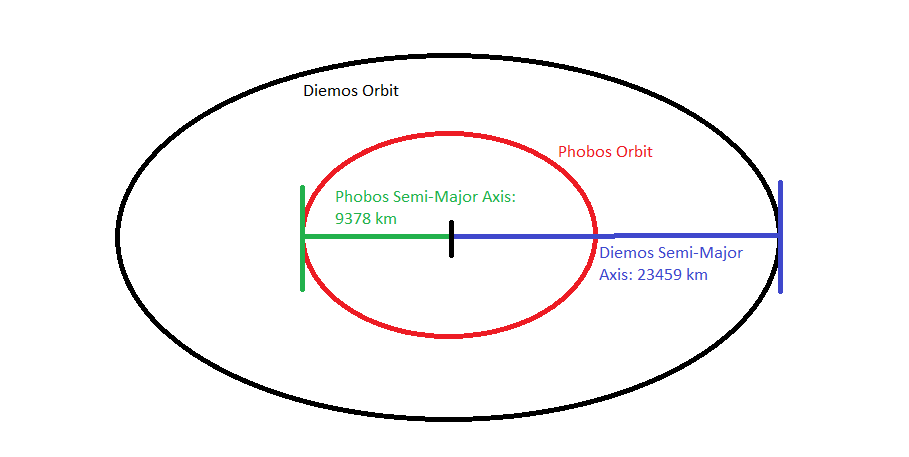
\includegraphics[width=1.0\textwidth, angle =0]{../images/semi-major-axis}
  \caption{A depiction of the semi-major axis of both Phobos and Demimos}
  \label{fig:semi-major-axis}
\end{figure}




% Do ALL math derivations here...label each equation and reference the
% equations accordingly... For example:  From Eq. (2), we see that Eqs. (3) - (7) 
% can be simplified, blah, blah...
\section{Theory}

\noindent The first step in solving for the system's X and Y coordinates involves calculating a relative Gravitational Constant for each moon. 

\begin{equation}
\label{eq:gravConstant}
 G = 4\pi ^{2}*\frac{R^{3}}{Year_{Moon}*M_{System}}~.
\end{equation}

\noindent Where $R$ is the semi-major axis, $Year_{Moon}$ is a time in seconds, and $M_{System}$ is the total mass of the Mars and the considered Moon, the following values may be plugged in and calculated:

\begin{table}[ht]
  \centering
  \begin{tabular}{|r|c|c|c|c|}
  \hline
                             & $R_{Moon}  (m)$  &  $Year_{Moon} (s)$ & $Mass (kg)$ & $Gravity  (N*m^{2}*kg^{-2})$ \\ \hline
  Phobos                 & $9.378*10^{6}$  & $27553.82$ &  $10.6*10^{15}$ & $4.2887*10^{13}$ \\ \hline
  Deimos 		     & $23.459*10^{6}$  & $109074.81$ &  $2.4*10^{15}$ & $4.283910*10^{13}$   \\ \hline
  Mars		     &                             &                    & $6.4171*10^{23}$  &\\ \hline
  \end{tabular}
  \label{table:lunar-properties}
  \caption{More Lunar Properties of The Moons as described by NASA~\cite{nasa}}
\end{table}

\noindent While the initial position doesn't need to be calculated due to our known semi-major axis. The initial velocity can be solved by equating the following two equations:

\begin{equation}
\label{eq:netForce}
 F_{Net}=\frac{M_{Moon}*v^{2}}{R}
\end{equation}

\begin{equation}
\label{eq:gravForce}
 F_{Gravity}=\frac{G_{Moon}}{R^{2}}
\end{equation}

\noindent Solving for velocity gives you the equation:

\begin{equation}
\label{eq:velocity}
V_{Moon} = \sqrt{\frac{Gravity_{Moon}}{R_{Moon}}}
\end{equation}

\noindent For every equation, you need to explain each variable, for example:

\begin{equation}
\label{eq:force}
F=\dfrac{mv^2}{r}~.
\end{equation}
\noindent In Eq.~\eqref{eq:force}, $F$ is the force measured in Newtons, $m$ is the
mass in kilograms, $v$ is the velocity measured in meters per second, and $r$ is
the radius of the curved path.  Equation~\eqref{eq:force} was obtain from~\cite{uni}.

\section{Computational Methods \& Techniques}
\noindent Once Parameter Calculations are completed the $(x, y)$ coordinates of the satelites must then be calculated using Runge Kutta systems ~\eqref{eq:rk2} and ~\eqref{eq:rk4}. This is a simple step summation used to simulate integration by properties of the right hand rule described as:

\begin{equation}
\label{eq:rhr}
\sum_{t=0}^{year}y(t)*dt
\end{equation}

\noindent The steps of Runge Kutta RK1-RK4 are as follows:

\begin{equation}
\label{eq:rk1}
k_{1}= \Delta t\vec{f}(\vec{y}^{n},t)
\end{equation}

\begin{equation}
\label{eq:rk2}
k_{2}= \Delta t\vec{f}(\vec{y}^{n} + \frac{1}{2}k_{1},t + \frac{1}{2}\Delta t)
\end{equation}

\begin{equation}
\label{eq:rk3}
k_{3}= \Delta t\vec{f}(\vec{y}^{n} + \frac{1}{2}k_{2},t + \frac{1}{2}\Delta t)
\end{equation}

\begin{equation}
\label{eq:rk4}
k_{4}= \Delta t\vec{f}(\vec{y}^{n} + k_{3}, t + \Delta t)
\end{equation}

\noindent In these differential systems the included calculation of the previous level show each step of the approximation system. From a basic vector in ~\eqref{eq:rk1} from the given condition, you then have a continuation off of the trajectory as ~\eqref{eq:rk2}. A better midpoint may then be calculated using ~\eqref{eq:rk3} (usually falling on the other side of the curve as ~\eqref{eq:rk2}) and ~\eqref{eq:rk4} shows a significant increase in accurace compared to just ~\eqref{eq:rk2}.

\section{Results}
\noindent While the primary printout of the results can be found in a data file containing approximately 100,000 data points, the full orbits can be seen visually in Fig. ~\ref{fig:orbit-diagram}.
\begin{figure}[ht]
\centering
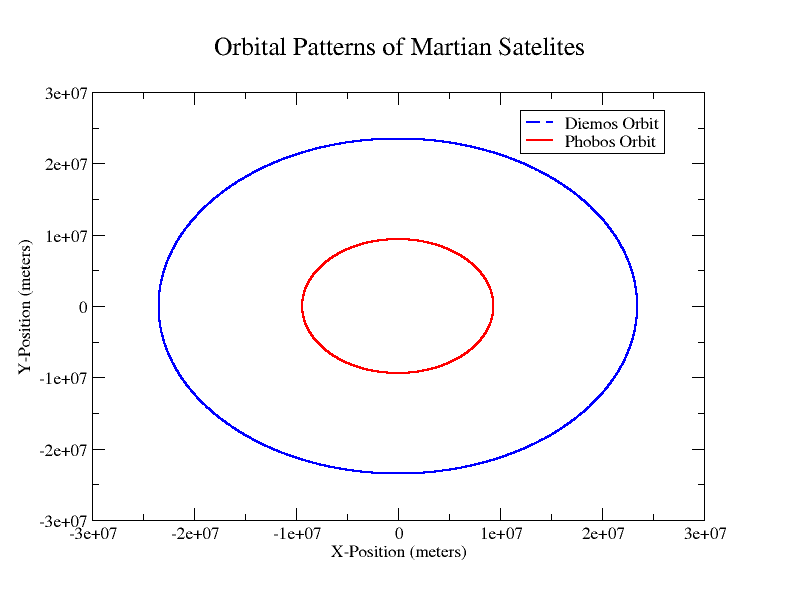
\includegraphics[width=1.0\textwidth, angle =0]{../images/orbits}
\caption{Orbital period in the $x-y$ plane for one full orbit of Phobos and Deimos orbiting Mars.}
\label{fig:orbit-diagram}
\end{figure}

\noindent With Mars at position $(0,0)$ in this system both orbits can be seen to have quite clean elliptical patterns. They look so perfect that you would assume that there would be more interference between the two of them having a two large satelites orbiting the same planet.

\section{Conclusions}
\noindent  The first check we can do is to make sure the energy in the system is conserved. By adding the Kinetic and Potential energy at each point for both systems we can get a figure of total energy over time. 

\begin{figure}[ht]
\centering
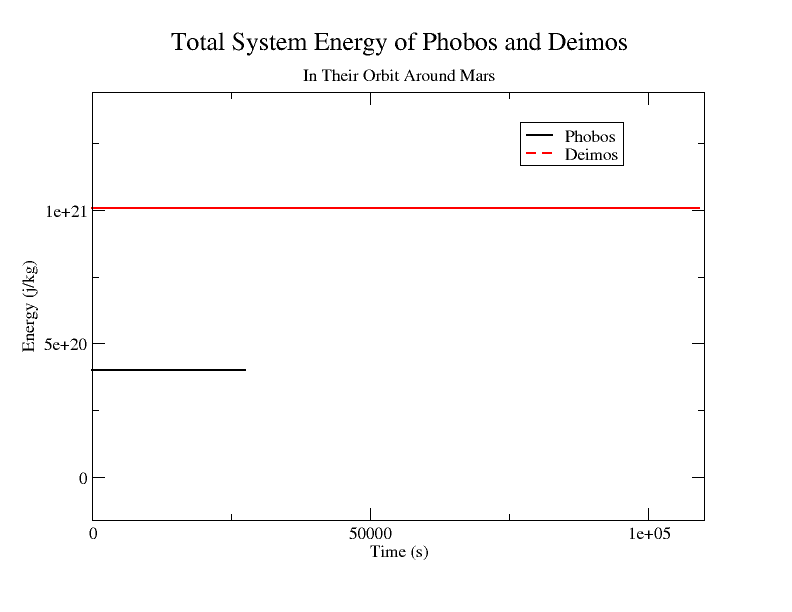
\includegraphics[width=1.0\textwidth, angle =0]{../images/energy}
\caption{Total Energy of Phobos and Deimos over time.}
\label{fig:energy}
\end{figure}

\noindent What we find is that our systems must be correct as the total energy in the systems remain constant; following a standard gravitational constant formula with the masses removed such as:

\begin{equation}
\label{relGravity}
acceleration = \frac{G}{R^2}
\end{equation}

\noindent where $G$ is the universal gravitational constant $6.67*10^-11 (N^{-11}*m^{3}*kg^{-1}*s^{-2}$, and the distance between them being their closest point at the semi-major axis where they are less affected by the planet $R = Semi-Major_{Deimos}-Semi-Major_{Phobos}$ the acceleration developed is still only about $4.73*10^{-15}$ Which explains why energy is conserved in the system.




\begin{thebibliography}{99}

\bibitem{uni} 
Douglas C. Giancoli
\textit{Physics for Scientists and Engineers}. 
Pearson Education Inc., Upper Saddle River, New Jersey, 2009.

\bibitem{nasa} 
NASA
\textit{Mars Fact Sheet}. 
NASA, 2016
nssdc.gsfc.nasa.gov/planetary/factsheet/marsfact.html

\end{thebibliography}




\end{document}